\chapter{Numerical methods to simulate dispersed phase}
\label{ch3:disperse_phase_methods}

\section{Introduction}

The previous chapter presented numerical methodologies applicable to separate two-phase flows. These are useful for solving problems where the dynamics of atomization need to be accurately resolved. Nonetheless, those methods cannot be applied in the dispersed phase regime, where atomization is complete (or almost complete) and a spray composed of individual droplets is formed. Such problems, often found when studying reactive processes where fuel is injected into a combustion chamber, need a different representation of the liquid phase so that 1) the spray can be transported with acceptable computational costs and 2) can include more complex physics relevant to reactive problems, such as evaporation and combustion.

The spray generated in the dispersed phase regime is mainly distinguished from liquid in the separate regime by the following features (represented in Figure \ref{fig:atomization_regimes_herrmann}):

\begin{itemize}

	\item The characteristic length scales of the particles. In dispersed phase flows, these ones are low and usually smaller than the resolution of the main grid.
	
	\item The value of the liquid volume fraction $\alpha_l$. In dispersed phase flows, $\alpha_l < 1$. According its value, one can distinguish between dense regime (moderate values of $\alpha_l$, particles are close to each other) and dilute regime (lower values of $\alpha_l$, usually below $10^{-3}$, particles are far from each other).

\end{itemize}

The numerical formalisms to resolved dispersed phase flows will hence depend on these two characteristics. It is also important to consider the interaction with the gaseous phase, since this one will depend by the resolution of the main grid. The interaction between the liquid and gaseous phases in dispersed phase flows can be quantified by means of the Stokes number $St$, defined as the ratio between the characteristic time-scale of a liquid particle $\tau_p$ and a characteristic time of the gaseous phase $\tau_g$: 

\begin{equation}
\label{eq:Stokes_number_definition_general}
St = \frac{\tau_p}{\tau_g}
\end{equation}

A classification of numerical methods to simulate dispersed phase flows based on the volume fraction and the Stokes number has been done by \citeColor[balachandar_scaling_2009], shown in Figure \ref{fig:balachandar_numerical_methods_representation}. As it can be seen, the Stokes number will depend on the numerical methodology used to resolve the gaseous phase: in DNS, the smallest scales of turbulence with characteristic size $\upeta$ will be resolved and will have a characteristic time $\tau_k$, while in LES the smallest scales resolved $\upxi$ will be larger and their time-scales will be different ($\tau_\upxi$). Regarding the volume fraction, coupling strategies between liquid particles and gas can be used depending on its value: in the dilute regime particles are far from each other and the interactions among them can be neglected (one and two-way coupling), while in the dense regime the interaction between particles must be taken into account (four-way coupling). The difference between one and two-way coupling depends on if the influence of the liquid phase onto the gas is considered with source terms (two-way coupling) or if it is neglected, so that the gaseous phase will not be perturbed by the particles (one-way coupling).


\begin{figure}[h!]
	\centering
	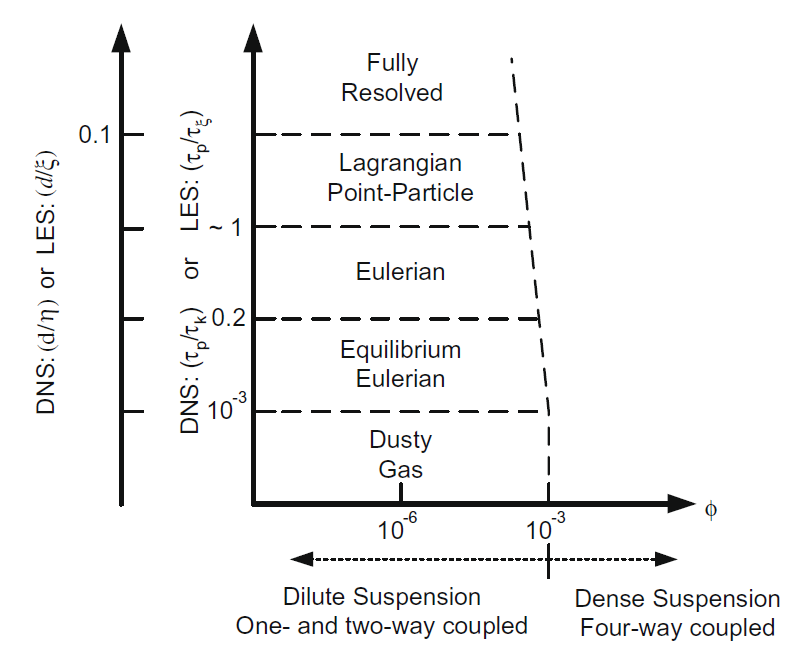
\includegraphics[scale=0.6]{./part1_numerical_approaches/figures_ch3/balachandar_disperse_phase_classification}
	\caption{Several numerical approaches to solve dispersed phase flows. Classification is done with respect to the liquid volume fraction (here defined as $\phi$) and to the Stokes number or, equivalently, to the ratio of largest to smallest length scales, which depend on the numerical resolution.  Source: \citeColor[balachandar_scaling_2009]}
	\label{fig:balachandar_numerical_methods_representation}
\end{figure}


\section{Numerical approaches to model dispersed phase flows}




Several approaches exist to study disperse phase. 



%\section{Spray characterisation (??)}

%Maybe this can be a subsection of the next section ?

In this chapter, 

\subsection{Spray representation}

A spray composed of dispersed droplets can be characterized by means of a number density function $f$. This function depends on time $t$, space $\textbf{x}$, velocity $\textbf{v}$ and radius $r$, and can be expressed as follows (\textbf{ref:2000-subramanian}):

\begin{equation}
f \left( t, \textbf{x}, \textbf{v}, r \right) = \sum_{p=1}^{N_d} \delta \left( \textbf{x} - \textbf{x}_p \left( t \right) \right)  \delta \left( \textbf{v} - \textbf{v}_p \left( t \right) \right) \delta \left( \textbf{r} - \textbf{r}_p \left( t \right) \right)
\end{equation}

where $N_d$ is the number of droplets in the spray, and $\textbf{x}_p$, $\textbf{v}_p$ and $r_p$ are each individual particles position, velocity and radius respectively. The function $f$ contains all the necessary information to represent the spray. The number of droplets in a spatial region $\left[ \textbf{x} + d\textbf{x} \right]$, 

By integrating the function $f$ one can obtain the density of droplets 


%The modeling of dispersed two-phase flows is based on a mesoscopic
%description of the dispersed phase. Particles are assumed to be spherical
%and fully characterized by a small set of variables: position x ,
%radius r (or more generally a size variable denoted by ϕ ), velocity v
%and temperature θ . In most applications, the particle number density
%function contains all the necessary information on the dispersed phase.
%By definition, f (t,x,r, v,θ )dxdrdvdθ denotes the averaged number
%of droplets with a size in [r,r + dr], a velocity in [v, v + dv], a temperature
%in [θ ,θ + dθ ] and located in the volume [x,x + dx] at time t .

\begin{equation}
\frac{\partial f}{\partial t} + \nabla_\textbf{x} \left( \textbf{v} f \right) + \nabla_\textbf{v} \left( \textbf{F} f \right) + \frac{\partial E_S f}{\partial S} + \frac{\partial E_T f}{\partial T}
\end{equation}

where $\textbf{x}$, $\textbf{v}$, $S$ and $T$ are each individual particle's position, velocity, surface and temperature, respectively; $F$ is the force acting on the particle, and $E_S$ and $E_T$ are respectively the exchange terms due to mass (evaporation rate) and energy (heat transfer).

Introduce the William-Boltzmann equation (2010 Vie, 20111 Murrone). 

\subsection{Direct approaches}

Make reference to Figure \ref{fig:balachandar_numerical_methods_representation}: fully resolved (FCM, 2010 Vie) and lagrangian point-particle (LPP or DPS, 2010 Vie). 

Explain that LPP will be used, and hence it will be discussed in $\S$\ref{sec:ch3_EL_formalisms}.




\subsection{Lagrangian point particle representation}
\label{sec:ch3_EL_formalisms}


The Lagrangian description (EL) does not use an averaging process in the grid for the fluid phase, but tracks each fluid particle individually. Every droplet is represented by its own equations which are not solved in the main grid (i.e. the Eulerian grid used to represent the carrier phase). This can make convergence difficult and hinders the introduction of parallelism techniques. However, the resulting system of equations is robust, the time per iteration is usually lower than for the EE description, and the drop-drop and drop-wall interactions are easier to model.

When considering droplets immersed in a gas, it is necessary to take into account mechanics of particle motion. A useful definition to study the relative influence between the droplet and the gas is the \textbf{Stokes number}, which is defined as the ratio between the characteristic time of the particle $\tau_p$ and the frequency of the flow fluctuations $f_{turb}$ around an obstacle \citepColor[koch_spray_2019]:

\begin{equation}
St = \tau_p f_{turb} = \frac{\tau_p \widetilde{\boldsymbol{u}}_g}{d_p}
\end{equation}

where $\widetilde{\boldsymbol{u}}_g$ is the gas velocity at the position of the particle $p$ assuming that the flow field is locally undisturbed by the presence of that particle. The Stokes number indicates how the droplet responds to fluctuations of the gas flow. If $St << 1$, the droplet will follow perfectly the fluctuations of the gas flow. On the contrary, if $St >> 1$ the droplets will rather neglect the flow trajectories and follow a ballistic trajectory. $\tau_p$ is obtained from the following expression (\textbf{CHECK THIS OUT}):


\begin{equation}
\tau_p = \frac{d_p^2 \rho_p}{18 \mu_\mathrm{g}} =  \frac{4}{3} \frac{\rho_p}{\rho_\mathrm{g}} \frac{d_p}{C_D | \boldsymbol{v}_r |} = \frac{4}{3} \frac{\rho_p d_{p^2}}{\mu_g Re C_D}
\end{equation}

For the description in the Lagrangian framework, each particle will be modelled according to the \textbf{Discrete Particle Simulations} (DPS) approach. DPS assumes each particle to be completely spherical and robust. With these assumptions, the \textbf{dynamic equations} for a particle $p$ in the spatial direction $i$ are:

\begin{subequations}
\label{eq:TPF_lagrange_dynamic_eqs}
\begin{align}
\frac{d \boldsymbol{x}_p}{d t} &= \boldsymbol{u}_p \\
\frac{d \boldsymbol{u}_p}{d t} &= \underbrace{ - \frac{3}{4} \frac{\rho_\mathrm{g}}{\rho_p} \frac{C_D}{d_p} | \boldsymbol{v}_r | \boldsymbol{v}_r }_{\text{Drag}\atop\text{term}}  + \underbrace{ \left( 1 - \frac{\rho_\mathrm{g}}{\rho_p} \right) \boldsymbol{g} }_{\text{Gravity}\atop\text{term}} 
\end{align}
\end{subequations}

% \frac{d u_{p,i}}{d t} &= \underbrace{ - \frac{3}{4} \frac{\rho_\mathrm{g}}{\rho_p} \frac{C_D}{d_p} | \boldsymbol{v}_r | v_{r,i} }_{\text{Drag}\atop\text{term}}  + \underbrace{ \left( 1 - \frac{\rho_\mathrm{g}}{\rho_p} \right) g_i }}_{\text{Gravity}\atop\text{term}} 

where $\rho_\mathrm{g}$ and $\rho_p$ are the gas and liquid particle densities respectively, $C_D$ is a drag coefficient, $d_p$ is the particle diameter, $\boldsymbol{v}_r$ is the relative velocity of the particle with respect to the airflow and $g$ is the gravity term. Equation (\ref{eq:TPF_lagrange_dynamic_eqs}b) is the momentum equation of the droplet and contains the contributions of the two forces considered: the drag force and the gravitational forces. The relative velocity is given by $\boldsymbol{v}_r = \boldsymbol{u}_p - \widetilde{\boldsymbol{u}}_g$ 

The drag coefficient $C_D$ is given by the following expression:

\begin{equation}
\label{eq:Re_CD_droplet}
C_D =
\left\{
    \begin{split}
     \frac{24}{Re} \left( 1 + 0.15 Re^{0.687} \right)\,\,\mathrm{if}\,\,Re < 1000 \\ 
    0.44\,\,\mathrm{if}\,\,Re \geq 1000 
    \end{split}
\right.
\end{equation}

where $Re = \rho_\mathrm{g} | \boldsymbol{v_r} | d_p / \mu_\mathrm{g} $. This expression was obtained experimentally by \citeColor[schiller_drag_1935] with the assumptions that the particles are perfectly spherical and rigid.  

%These assumptions also allow for the definition of the characteristic time of a particle $p$:

%\begin{equation}
%\tau_p = \frac{d_p^2 \rho_p}{18 \mu_\mathrm{g}} =  \frac{4}{3} \frac{\rho_p}{\rho_\mathrm{g}} \frac{d_p}{C_D | \boldsymbol{v_r} |} 
%\end{equation}

Besides the dynamic equations, it is also necessary to account for the \textbf{phase transition} of the liquid dispersed phase into gaseous phase. 

\begin{subequations}
\label{eq:TPF_lagrange_phasetransition_eqs}
\begin{align}
\frac{d m_p}{d t} &= \dot{m}_p = \Gamma \\
\frac{d h_p}{d t} &= \Phi_p
\end{align}
\end{subequations}

Equation (\ref{eq:TPF_lagrange_phasetransition_eqs}a) accounts for the \textbf{evaporation} process. If the uniform temperature model is used, then (\ref{eq:TPF_lagrange_phasetransition_eqs}) is equal to (\ref{eq:evaporation_mass_flow_rate}). Equation (\ref{eq:TPF_lagrange_phasetransition_eqs}b) accounts for the energy transfer. By considering the effects of the \textbf{conduction} and the \textbf{evaporation} processes in terms of energetic balance, $\Phi_p$ can be extended as follows:

\begin{equation}
\Phi_p = m_p C_{P_\mathrm{g}} \frac{d T_p}{d t} = \underbrace{ h_p \pi d_p^2 \left( T_\mathrm{g} - T_p \right) }_{\text{Conduction}\atop\text{term}} - \underbrace{ \dot{m}_p  \Delta h_v }_{\text{Evaporation}\atop\text{term}}
\end{equation}

where $C_{P_\mathrm{g}}$ is the gas specific heat capacity at constant pressure, $T_p$ is the particle temperature, $T_\mathrm{g}$ is the gas temperature, $h_p$ is the film coefficient of the gas at the particle surface and $\Delta h_v$ is the latent heat of vaporization of the particle. 

By considering Equations (\ref{eq:TPF_lagrange_dynamic_eqs}) and (\ref{eq:TPF_lagrange_phasetransition_eqs}) with all the simplifications stated, the final set of equations for the Lagrangian dispersed phase approach is:

\begin{subequations}
\begin{align}
\frac{d x_{p,i}}{d t} &= u_{p,i} \\
\frac{d u_{p,i}}{d t} &= - \frac{u_{p,i} - \widetilde{u}_{g,i} }{\tau_p} + \left( 1 - \frac{\rho_\mathrm{g}}{\rho_p} \right) g_i \\
\frac{d m_p}{d t} &= \Gamma \\
m_p C_{P_\mathrm{g}} \frac{d T_p}{d t} &= h_p \pi d_p^2 \left( T_\mathrm{g} - T_p \right) - \dot{m}_p  \Delta h_v
\end{align}
\end{subequations}

\subsection{Other approaches}

Mention eulereian methods (mesoscopic, quadrature, maybe also stochastic methods). Mention that they're out of the scope of this thesis. Comment statistical approaches ( 2000 SUbramanian, 2010 Vie, Vie 2013). Mention that they are out of the scope of this thesis, so we are gonna focus on EE and EL.


\section{Lagrangian injection models for multipoint injection}
\label{sec:ch3_state_art_lagrangian_injection}

A classification of models for liquid injection in dispersed phase computations is proposed in Figure \ref{fig:state_art_injection}. Each category has the following advantages and disadvantages (see presentation 2020 12 15):

\begin{itemize}

	\item \textbf{Based on empirical laws}. \textcolor{green}{Advantage}: embedded physics. \textcolor{red}{Disadvantage}: restricted to geometry and operating conditions of development.
	
	\item \textbf{Injection of fully developed spray}. \textcolor{green}{Advantage}: droplets size distributions directly imposed. \textcolor{red}{Disadvantage}: Primary atomization neglected.
	
	\item \textbf{Effect of dense spray in gaseous phase}. \textcolor{green}{Advantage}: in JICF, taking into account blockage effect. \textcolor{red}{Disadvantage}: None.
	
	\item \textbf{Addition of secondary atomization model}. Good if atomziation not present.
	
	\item \textbf{Reference spray learning}. So far, and to our knowledge, there are no available models that can use a reference spray to learn boundary conditions (droplet sizes, velocity distributions, spatial location of injectors) for dispersed phase computations. \textcolor{green}{Advantage}: Applicable to generic injectors and 
	wide range of operating conditions.  \textcolor{red}{Disadvantage}: Need of detailed spray characterisation from simulations or experiments.

\end{itemize}

%\begin{figure}[h!]
%	\centering
%	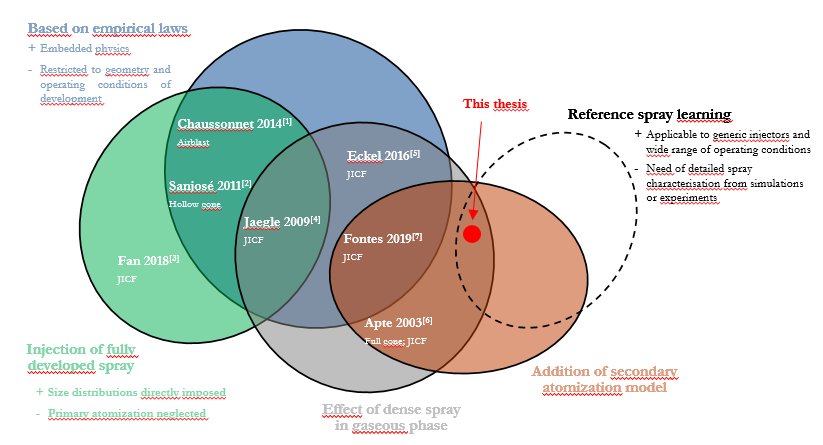
\includegraphics[scale=0.5]{./part1_numerical_approaches/figures_ch3/state_art_lagrangian}
%	\caption{Classification of lagrangian injection models}
%	\label{fig:state_art_injection}
%\end{figure}

\begin{figure}[h!]	
	\centering
	\includeinkscape[inkscapelatex=true,scale=0.75]{./part1_numerical_approaches/figures_ch3/state_art_lagrangian}
	\caption{Classification of lagrangian injection models}
	\label{fig:state_art_injection}
\end{figure}

\subsection{Airblast spray}

Basically Chaussonnet.

\subsection{Hollow cone spray}

Basically FIMUR.

\subsection{Liquid jet in crossflow}

Aqui viene el arsenal.